% !TeX root = ../thuthesis-example.tex

\chapter{实验与分析\label{sec:chap8}}
本章对前文中所提出的优化设计进行实验,验证这些设计的效果。本章首先介绍实验所使用的负载程序,包括一个负责对用户场景特点进行采样的负载采样程序和根据用户负载特征进行写入的模拟负载运行程序。本工作利用负载采样程序和模拟负载运行程序模拟了若干真实用户的负载,并与 IoT Benchmark\cite{liu2019benchmarking} 下的若干组配置一起构成了本工作的测试负载。接着,本章利用这组负载分别测试了压力测试和用户模拟负载测试场景下本文各部分工作的性能提升,最后测试了将所有优化措施相结合的性能提升。
\section{测试负载设计}
本节介绍实验所使用的负载采样程序和负载模拟程序的设计,并通过这些程序采样了一组真实用户的负载。在模拟真实用户的负载之外,测试负载还包括了使用 IoT Benchmark 所模拟的若干压力测试负载场景。这些负载一起构成了本工作的测试负载集。
\subsection{负载采样程序}
目前 IoTDB 一共有超过一千家企业用户,这些用户的写入负载特征各异。例如在车联网场景中,设备数通常非常多,每个设备产生数据的频率较低;在工业监控场景中,设备数则相对较少,但每个设备产生数据的频率有可能较高。在同一个场景中,不同设备的数据产生频率、时间序列类型、时间序列数量等也可能有所不同。因此,为了更好地模拟真实用户的负载,本工作设计了一个负载采样程序,用于对用户场景特点进行采样。

负载采样程序的主要功能是通过扫描用户运行 IoTDB 所产生的 TsFile,收集时间序列的特征信息。这些信息包括:
\begin{itemize}
  \item \textbf{不同时间序列类型的比例}:IoTDB 目前支持六种类型的时间序列,分别是 INT32、INT64、FLOAT、DOUBLE、BOOLEAN 和 TEXT。不同时间序列类型的比例对于写入性能有一定影响,例如 TEXT 类型写入需要消耗更大的内存,会产生较大的写前日志,而 BOOLEAN 类型的写入则资源消耗相对较小。
  \item \textbf{时间序列数据的频率分布}:不同时间序列的数据产生频率不同,有的时间序列数据产生频率较高,有的时间序列数据产生频率较低,这是用户负载一个重要的特征。
  \item \textbf{单个设备下时间序列数量的分布}:即使在同一用户场景下,不同设备下时间序列数量也可能相差较大,负载采样程序收集每个设备下时间序列数目的分布信息,为构建负载模拟程序提供参考。
  \item \textbf{对齐时间序列与非对齐时间序列的比例}:IoTDB 目前支持两种序列类型,分别是对齐时间序列和非对齐时间序列。两种时间序列在性能上有所不同,对齐时间序列的写入性能较高,而非对齐时间序列的写入性能较低。负载采样程序收集对齐时间序列和非对齐时间序列的比例信息,为构建负载模拟程序提供参考。
  \item \textbf{时间序列的数值分布}:时间序列数据的值分布对于压缩和编码算法性能有一定的影响,负载模拟程序采集不同数据类型的值分布,为构建负载模拟程序提供参考。
\end{itemize}

\begin{figure}
  \centering
  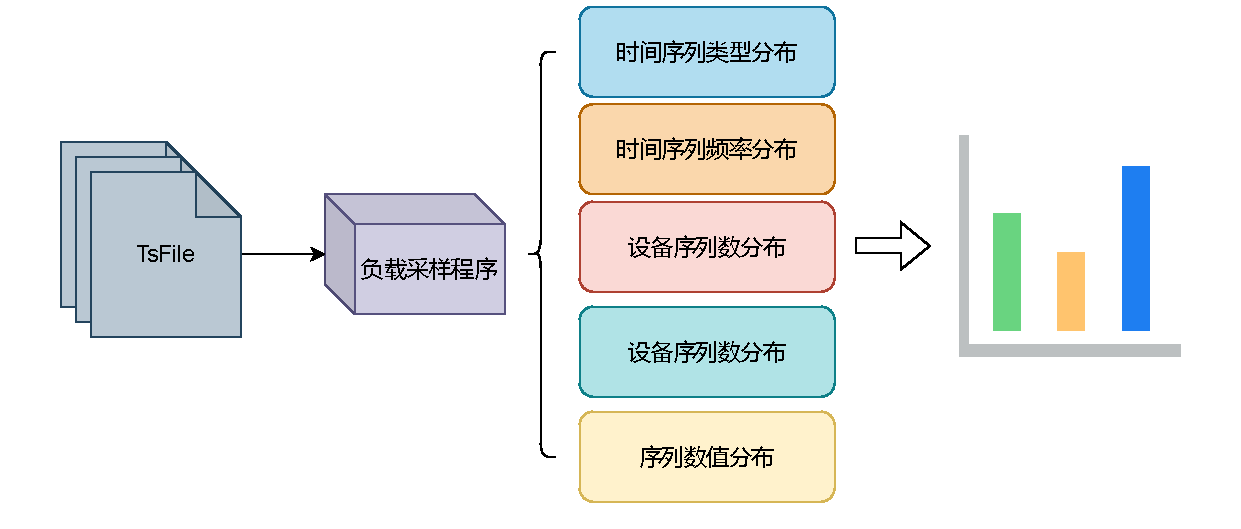
\includegraphics[width=\textwidth]{负载采样程序.pdf}
  \caption{负载采样程序架构}
  \label{fig:load-sampling-program}
\end{figure}

负载采集程序的输入是用户的 TsFile,TsFile 中的数据区分为多个数据块组(ChunkGroup),每个数据块组又分为多个数据块(Chunk)。一个数据块组就对应了一个设备,而一个数据块就对应了一个时间序列的数据。负载采样程序使用 IoTDB 所提供的 TsFileSequenceReader 顺序扫描 TsFile,通过读取每个数据块的数据类型来收集不同时间序列类型的比例,通过读取一个数据块中最大时间点与最小时间点的时间差除以数据点的数目来收集时间序列的频率分布,通过统计每个数据块组下数据块的数目来收集单个设备下时间序列数量的分布,通过读取每个数据块组的类型(对齐或非对齐)来收集对齐时间序列与非对齐时间序列的比例,通过读取每个数据块的数据值来收集不同类型时间序列的数值分布。最后,负载模拟程序将采集到的信息以直方图的形式输出为一个文件,供负载模拟程序使用。

\subsection{负载模拟程序}
图 \ref{fig:load-simulation-program} 展示了模拟负载程序的架构,模拟负载程序接收两个输入,一个是负载采样程序输出的直方图文件,另一个是负载的总设备数。模拟负载程序的运行主要分为两步,第一步是根据直方图和总设备数生成测试的时间序列和设备元数据,第二步则是根据时间序列和设备元数据模拟用户的写入请求。

\begin{figure}
  \centering
  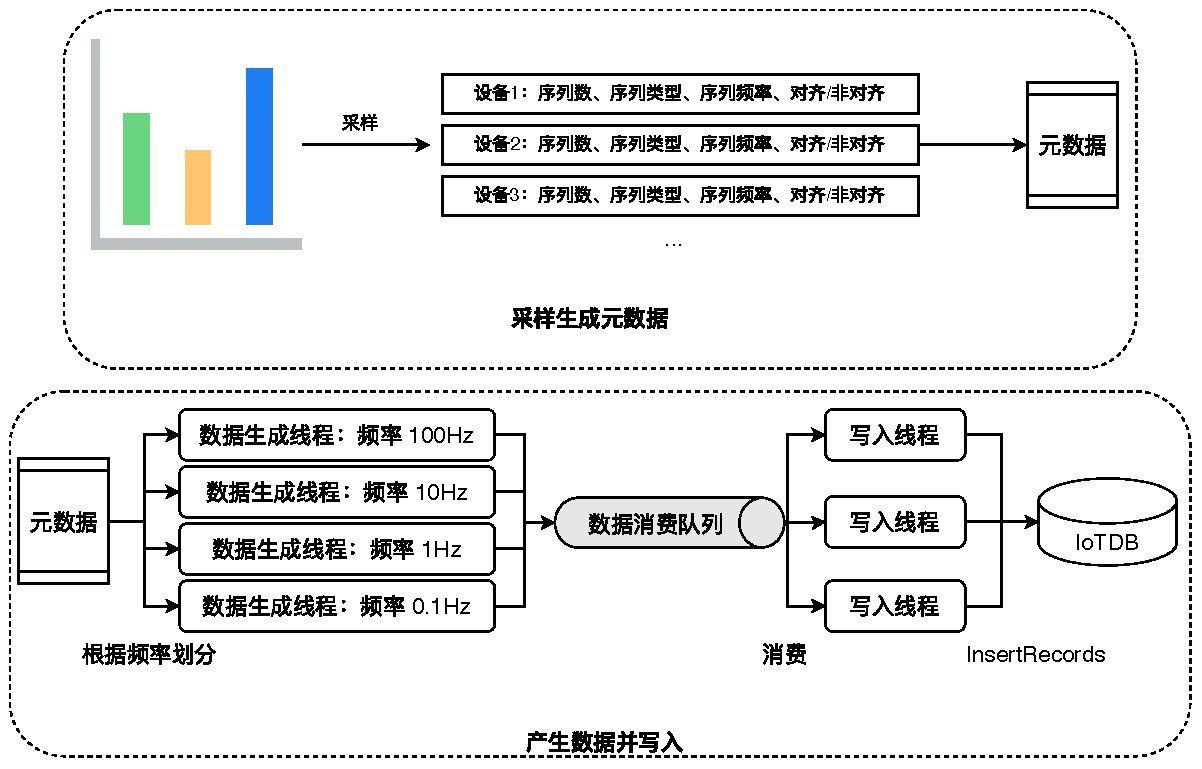
\includegraphics[width=\linewidth]{模拟负载运行程序.pdf}
  \caption{负载模拟程序架构}
  \label{fig:load-simulation-program}
\end{figure}

模拟负载程序运行的第一步是生成测试所需的元数据,这里的元数据既包含了在 IoTDB 中注册时间序列所需的信息,如每个设备下的序列数、序列名称、序列类型,也包含了模拟程序产生数据点所需的信息,如序列的频率、序列的值分布。这些数据的产生通过按照直方图中的分布随机采样得到。一个设备首先会先根据对每个设备下时间序列数的分布进行随机采样,得到本设备的序列数,然后再对频率直方图采样得到本设备下所有时间序列的数据生成频率。然后对于本设备下的每个时间序列,再采样得到其数据类型、值分布等。最后,模拟负载程序一方面将时间序列的元数据注册到 IoTDB 中,另一方面也会将这些信息保存在内存中,用于后续模拟数据的生成和写入。

模拟负载程序运行的第二步是模拟用户的写入请求。模拟负载程序首先会将第一步中生成的设备按照产生数据的频率进行划分,相同频率的设备被归类到一起。然后,具有相同频率的设备会被放到同一个数据生成线程中,这个线程会按照这批设备的频率周期性地按照每个设备的值分布产生数据。如果某一个频率的设备数过多,使用一个线程有可能导致无法按照规定的周期产生数据。例如,如果有大量 100 Hz 的设备,理论上每个设备每隔 10 ms 就要产生一批数据,但是一个线程有可能无法在 10 ms 内产生所有设备的数据,这就会导致最终设备生成数据的频率小于 100 Hz。为了避免这样的情况,每个线程最多负责 5000 个设备的数据生成。这样,即使设备数较多,也可以保证每个设备的数据生成频率不会受到影响。每个数据生成线程会将周期性产生的数据放入一个有限大小的内存并发队列中等待写入线程的消费,如果队列满了就会放弃将数据放入队列,并通过日志记录这种情况。写入队列会不断地从队列中取出数据并在本地缓存生成一个写入请求,如果写入请求的记录行数超过 2000 条或者该写入请求中最旧的数据点的时间戳距离当前时间超过 10 秒,就会将该写入请求通过 \emph{insertRecords} 接口写入到 IoTDB 中。写入线程的数量可以进行调节,以模拟不同的场景。在这样的设计下,模拟负载程序可以容忍 IoTDB 一定的写入延迟波动,从而更好地模拟真实用户的负载。
\subsection{测试负载描述}
利用负载采样程序和负载模拟程序,我们分析了中冶赛迪、四维智联、宝武钢铁集团、长安汽车四家用户的负载,构建了这四家用户的模拟负载程序。这四家用户的负载特征如图 \ref{fig:zysd-load-feature}、图 \ref{swzl-load-feature}、图 \ref{bwgt-load-feature}、图 \ref{caqc-load-feature} 所示。

此外,我们使用了 IoT Benchmark 对数据库的极限性能进行测试。我们可以通过配置 IoT Benchmark 的配置来实现模拟不同环境下的压力测试,我们分别模拟了常规设备数序列数场景、海量设备场景、海量序列场景。这三个场景所对应的配置如表 \ref{tabular:iot-benchmark-config} 所示。在使用 IoT Benchmark 进行压力测试时,不同类型的时间序列数量相同的,每个设备下的时间序列数也是相同的。写入线程在将数据写入到数据库之后,会马上进行下一次写入。因此,理论上每个时间序列产生数据的频率是非常大的,完全取决于数据库写入的延迟。在这种情况下,IoT Benchmark 可以模拟出一个极限的写入场景,测试出数据库的极限写入性能。

\begin{table}
  \centering
  \caption{IoT Benchmark 压力测试配置}
  \begin{tabular}{lllll}
    \toprule 
    场景 & 设备数 & 时间序列数 & 总时间序列数 & 存储组数  \\
    \midrule 
    常规设备数序列数场景 & 100000 & 20 & 2,000,000 & 5  \\
    海量设备场景 & 1000000 & 10 & 10,000,000 & 5  \\
    海量序列场景 & 10000 & 2000 & 20,000,000 & 5  \\
    \bottomrule
  \end{tabular}
  \label{tabular:iot-benchmark-config}
\end{table}


\section{客户端数据预处理性能测试}
\section{写入请求列示序列化性能测试}
\section{存储引擎执行优化性能测试}
\section{综合性能测试}
\subsection{压力性能测试}
\subsection{用户模拟负载测试}
\section{本章小结}